\chapter{Perancangan}
\label{chap: perancangan}
	
	Pada bab ini akan dijelaskan mengenai perancangan aplikasi yang dibangun meliputi perancangan kelas, \textit{routes}, \textit{controllers}, \textit{models}, perancangan antarmuka.
	
	\section{Perancangan Kelas}
	\label{sec: rancangKelas}
	
	Seperti yang sudah di jelaskan pada bab sebelumnya, untuk memodelkan sistem penilaian sidang skripsi 2 dengan menggunakan \textit{codeigniter} membutuhkan \textit{routes}, \textit{controllers}, \textit{models}, dan \textit{views}. Hal-hal berikut akan dijelaskan pada subbab selanjutnya.
	
	\section{Routes}
	\label{sec: routes}
	
	\textit{Routes} merupakan bagian dari \textit{codeigniter} untuk melakukan pemetaan terhadap lokasi \textit{file controllers} dari aplikasi. Berikut adalah isi dari "config/routes":
	\begin{lstlisting}[caption= File Routes, label= routes]
		$route['default_controller'] = 'C_skripsi';
		$route['404_override] ="";
		$route[translate_url_dahses'] =	FALSE;
	\end{lstlisting}
	Baris pertama dari Listing \ref{routes} di atas adalah nama \textit{file controller} yang terletak di \textit{folder controllers} yang akan diambil. Baris kedua merupakan kode untuk menangani \textit{error} yang terjadi jika \textit{file} yang dicari tidak ditemukan, contoh penggunaanya adalah "\$route['404\_override'] = 'errors/page\_missing;". Baris ketiga mempunyai fungsi mengganti seluruh nama \textit{file} yang mengandung '-' menjadi '\_', contoh penggunaanya adalah: "my-controller/index"	menjadi "my\_controller/index".

	\section{Controllers}
	\label{sec: controllers}
	
	\textit{Controller} terdiri dari sebuah kelas yang dinamakan "C\_Skripsi". Keseluruhan aktivitas dari sistem informasi penilaian skripsi diatur oleh kelas ini. Seperti yang telah dibahas pada Gambar \ref{fig:controllers}, berikut ini adalah \textit{file controller} dengan nama C\_skripsi.php.
	
	\begin{lstlisting}[caption= File Controller, label= ciController]
		<?php
		defined('BASEPATH') OR exit('No direct script access allowed');
		
		class C_skripsi extends CI_Controller {
		
		public function index()
		{
			$this->load->view('skripsi');
		}
		
		public function tambahDataMahasiswa(){
			$semester = $_POST['semester'];
			$tahun = $_POST['tahun'];
			$npm = $_POST['npm'];
			$nama = $_POST['nama'];
			$judul = $_POST['judul'];
			$namaPembimbing = $_POST['namaPembimbing'];
			$namaPembimbingPendamping = $_POST['namaPembimbingPendamping'];
			$namaKetuaTimPenguji = $_POST['namaKetuaTimPenguji'];
			$namaAnggotaTimPenguji = $_POST['namaAnggotaTimPenguji'];
			$bobotKetuaTimPenguji = $_POST['bobotKetuaTimPenguji'];
			$bobotAnggotaTimPenguji = $_POST['bobotAnggotaTimPenguji'];
			$bobotPembimbing = $_POST['bobotPembimbing'];
			$nilaiKoordinatorSkripsi = $_POST['nilaiKoordinatorSkripsi'];
			$bobotKoordinatorSkripsi = $_POST['bobotKoordinatorSkripsi'];
			$bobotTataTulisLaporanAnggota = $_POST['bobotTataTulisLaporanAnggota'];
			$bobotKelengkapanMateriAnggota = $_POST['bobotKelengkapanMateriAnggota'];
			$bobotPenguasaanMateriAnggota = $_POST['bobotPenguasaanMateriAnggota'];
			$bobotPresentasiAnggota = $_POST['bobotPresentasiAnggota'];
			$bobotPencapaianTujuanAnggota = $_POST['bobotPencapaianTujuanAnggota'];
			$bobotTataTulisLaporanKetua = $_POST['bobotTataTulisLaporanKetua'];
			$bobotKelengkapanMateriKetua = $_POST['bobotKelengkapanMateriKetua'];
			$bobotPenguasaanMateriKetua = $_POST['bobotPenguasaanMateriKetua'];
			$bobotPresentasiKetua = $_POST['bobotPresentasiKetua'];
			$bobotPencapaianTujuanKetua = $_POST['bobotPencapaianTujuanKetua'];
			$bobotTataTulisLaporanPembimbing = $_POST['bobotTataTulisLaporanPembimbing'];
			$bobotKelengkapanMateriPembimbing = $_POST['bobotKelengkapanMateriPembimbing'];
			$bobotPenguasaanMateriPembimbing = $_POST['bobotPenguasaanMateriPembimbing'];
			$prosesBimbinganPembimbing = $_POST['prosesBimbinganPembimbing'];
			$nilaiAkhirMahasiswa = $_POST['nilaiAkhirMahasiswa'];
			$data_insert = array(
				'semester' => $semester,
				'tahun' => $tahun,
				'npm' => $npm,
				'nama' => $nama,
				'judul' => $judul,
				'namaPembimbing' => $namaPembimbing,
				'namaPembimbingPendamping' => $namaPembimbingPendamping,
				'namaKetuaTimPenguji' => $namaKetuaTimPenguji,
				'namaAnggotaTimPenguji' => $namaAnggotaTimPenguji,
				'bobotKetuaTimPenguji' => $bobotKetuaTimPenguji,
				'bobotAnggotaTimPenguji' => $bobotAnggotaTimPenguji,
				'bobotPembimbing' => $bobotPembimbing,
				'nilaiKoordinatorSkripsi' => $nilaiKoordinatorSkripsi,
				'bobotKoordinatorSkripsi' =>$bobotKoordinatorSkripsi,
				'bobotTataTulisLaporanAnggota' => $bobotTataTulisLaporanAnggota,
				'bobotKelengkapanMateriAnggota' => $bobotKelengkapanMateriAnggota,
				'bobotPenguasaanMateriAnggota' => $bobotPenguasaanMateriAnggota,
				'bobotPresentasiAnggota' => $bobotPresentasiAnggota,
				'bobotPencapaianTujuanAnggota' => $bobotPencapaianTujuanAnggota,
				'bobotTataTulisLaporanKetua' => $bobotTataTulisLaporanKetua,
				'bobotKelengkapanMateriKetua' => $bobotKelengkapanMateriKetua,
				'bobotPenguasaanMateriKetua' => $bobotPenguasaanMateriKetua,
				'bobotPresentasiKetua' => $bobotPresentasiKetua,
				'bobotPencapaianTujuanKetua' => $bobotPencapaianTujuanKetua,
				'bobotTataTulisLaporanPembimbing' => $bobotTataTulisLaporanPembimbing,
				'bobotKelengkapanMateriPembimbing' => $bobotKelengkapanMateriPembimbing,
				'bobotPenguasaanMateriPembimbing' => $bobotPenguasaanMateriPembimbing,
				'prosesBimbinganPembimbing' => $prosesBimbinganPembimbing,
				'nilaiAkhirMahasiswa' => $nilaiAkhirMahasiswa,
		
			);
			$res = $this->skripsi_model->insertDataMahasiswa('beritaacarasidangskripsi',$data_insert);
			redirect(base_url(), 'refresh');
		}
		
		}
	\end{lstlisting}
	
	Keterangan Listing \ref{ciController}.
	\begin{itemize}
		\item public function index()\\
		Berfungsi untuk mengarahkan pengguna ke \textit{file views default} dari aplikasi.
		\item public function tambahDataMahasiswa()\\
		Berfungsi untuk mengambil data dari \textit{view} yang tersedia, untuk kemudian diolah menjadi bahasa sql oleh \textit{models}.
	\end{itemize}
	
	\section{Models}
	\label{sec: models}
	
	\textit{Models} mempunyai fungsi menghubungkan \textit{views} dan \textit{controllers} pada basis data. Pada penggunaan \textit{codeigniter}, \textit{model} dibuat dengan sangat sederhana. Berikut adalah isi dari kelas model:
	\begin{lstlisting}[caption= File Model, label= models]
		<?php
			defined('BASEPATH') OR exit('No direct script access allowed');
			
			class Skripsi_model extends CI_Model {
			
			public function insertDataMahasiswa($tableName, $data){
				$res = $this->db->insert($tableName, $data);
			}
		}
		
	\end{lstlisting}
	\textit{Method} pada Listing \ref{models}:
	\begin{itemize}
		\item public function insertDataMahasiswa(\$tablename, \$data)\\
		Berfungsi untuk mengolah data yang sudah diolah oleh \textit{controllers} menjadi kueri sql \textit{insert data}.
	\end{itemize}
	
	\section{Perancangan Basis Data}
	\label{sec: perancanganDatabase}
	
	Berdasarkan analisis basis data pada bab \ref{sub: analisisDatabase}, maka dibuat tabel basis data.
	\begin{table}[H]
	\centering
	\caption{Tabel Perancangan Basis Data}
	\begin{tabular}{| m{0.75cm} | m{7cm} | m{3cm} |}
		\hline
		No & Nama Tabel & Jenis Data\\
		\hline
		1 & \underline{id} & int(11)\\
		\hline
		2 & tahun & year(4)\\
		\hline
		3 & semester & int(1)\\
		\hline
		4 & npm & varchar(10)\\
		\hline
		5 & nama & varchar(256)\\
		\hline
		6 & judul & varchar(256)\\
		\hline
		7 & namaPembimbing & varchar(256)\\
		\hline
		8 & namaPembimbingPendamping & varchar(256)\\
		\hline
		9 & namaKetuaTimPenguji & varchar(256)\\
		\hline
		10 & namaAnggotaTimPenguji & varchar(256)\\
		\hline
		11 & bobotKetuaTimPenguji & int(2)\\
		\hline
		12 & bobotAnggotaTimPenguji & int(2)\\
		\hline
		13 & bobotPembimbing & int(2)\\
		\hline
		14 & nilaiKoordinatorSkripsi & float\\
		\hline
		15 & bobotKoordinatorSkripsi & int(2)\\
		\hline
		16 & bobotTataTulisLaporanAnggota & int(2)\\
		\hline
		17 & bobotKelengkapanMateriAnggota & int(2)\\
		\hline
		18 & bobotPenguasaanMateriAnggota & int(2)\\
		\hline
		19 & bobotPresentasiAnggota & int(2)\\
		\hline
		20 & bobotPencapaianTujuanAnggota & int(2)\\
		\hline
		21 & bobotTataTulisLaporanKetua & int(2)\\
		\hline
		22 & bobotKelengkapanMateriKetua & int(2)\\
		\hline
		23 & bobotPenguasaanMateriKetua & int(2)\\
		\hline
		24 & bobotPresentasiKetua & int(2)\\
		\hline
		25 & bobotPencapaianTujuanKetua & int(2)\\
		\hline
	\end{tabular}
\end{table}
\begin{table}[H]
\centering
	\begin{tabular}{| m{0.75cm} | m{7cm} | m{3cm} |}
	\hline
		26 & bobotTataTulisLaporanPembimbing & int(2)\\
		\hline
		27 & bobotKelengkapanMateriPembimbing & int(2)\\
		\hline
		28 & bobotPenguasaanMateriPembimbing & int(2)\\
		\hline
		29 & prosesBimbinganPembimbing & int(2)\\
		\hline
		30 & nilaiAkhirMahasiswa & float\\
		\hline
		\end{tabular}
	\end{table}
	
	\section{Perancangan Tampilan}
	\label{sec: perancanganTampilan}
	
	Tampilan pada sistem informasi penilaian skripsi haruslah dibuat semirip mungkin dengan form penilaian skripsi yang sudah ada seperti pada lampiran gambar \ref{fig: skripsiAsli} dan gambar \ref{fig: rekapAsli}.
	
	Perbedaan yang akan ditampilkan adalah dengan adanya otomatisasi penghitungan nilai sesuai dengan bobot yang diberikan kepada penilai. Hal ini akan memberikan kemudahan penilai untuk melakukan penilaian.
	
	Gambar \ref{fig:beritaacara} adalah bayangan awal tampilan untuk sistem informasi penilaian skripsi lembar berita acara sidang skripsi.
	\begin{figure}[H]
		\centering
		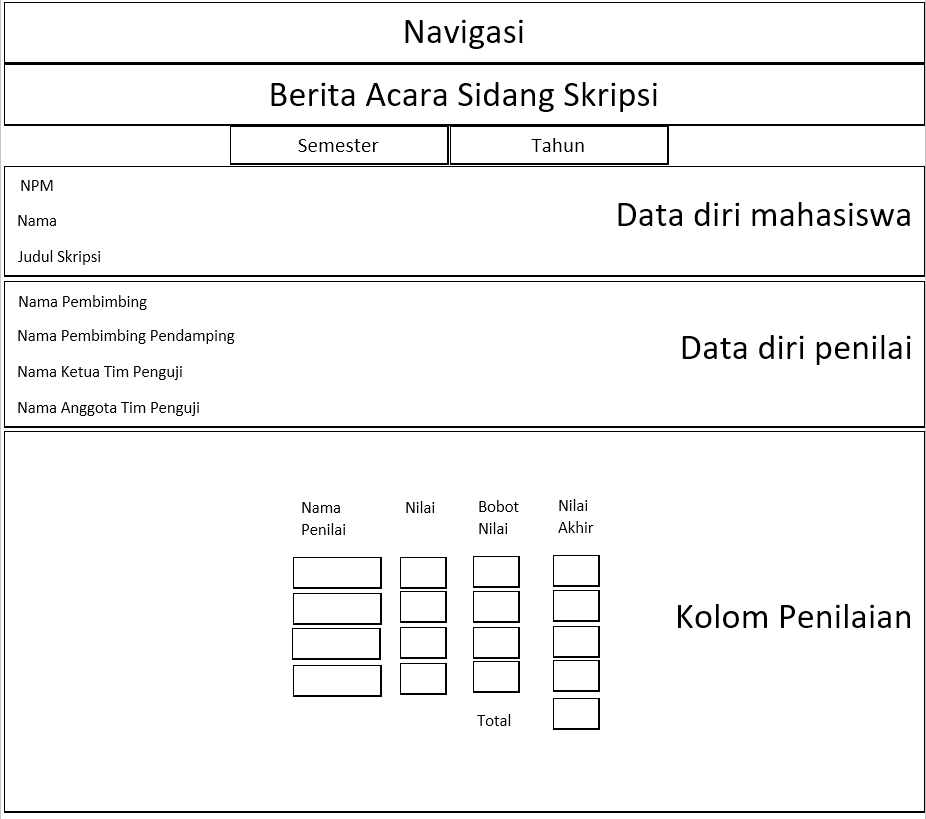
\includegraphics[scale=0.75]{Gambar/beritaacara}
		\caption{Perkiraan Tampilan Lembar Berita Acara Sidang Skripsi}
		\label{fig:beritaacara}
	\end{figure}

	Gambar \ref{fig:rekapitulasi} adalah bayangan awal tampilan untuk sistem informasi penilaian skripsi lembar rekapitulasi ketua tim penguji, anggota tim penguji, dan pembimbing.
	\begin{figure}[H]
		\centering
		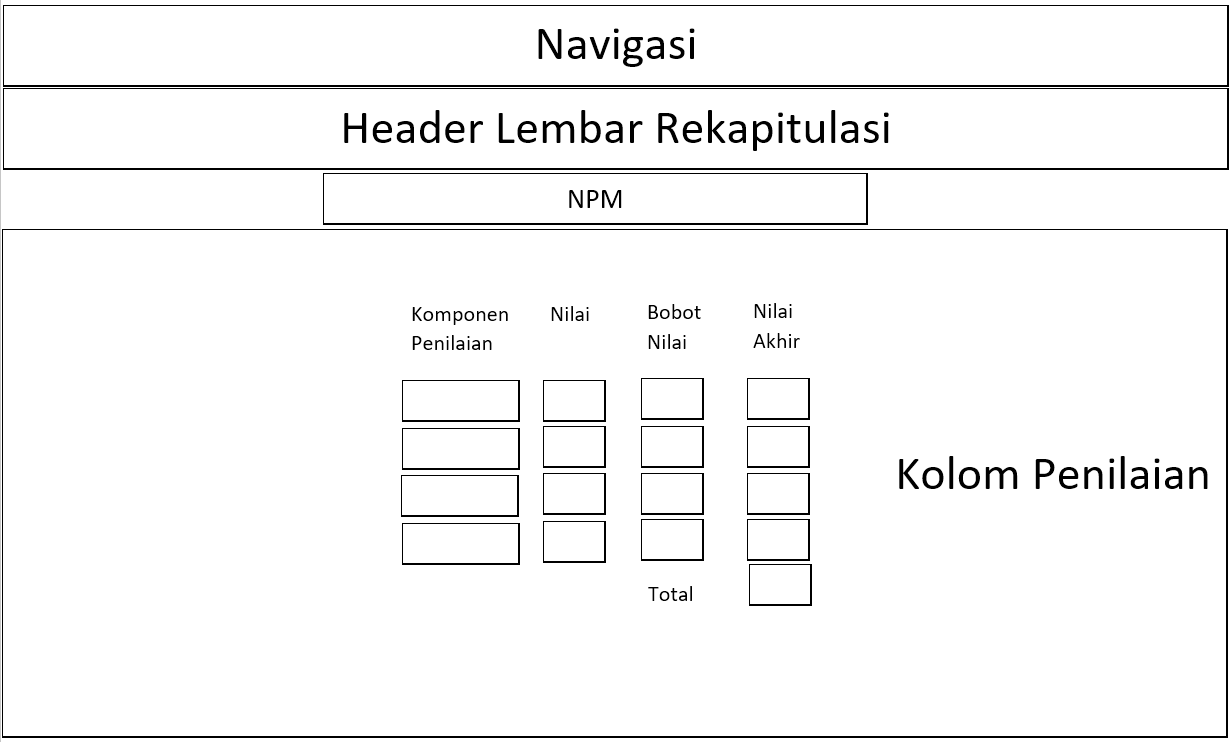
\includegraphics[scale=0.5]{Gambar/rekapitulasi}
		\caption{Perkiraan Tampilan Lembar Rekapitulasi}
		\label{fig:rekapitulasi}
	\end{figure}